\section{Collision probabilities}

So far, we have only dealt with homogeneous systems and the effect of energy self-shielding. However, spatial self-shielding is extremely important and we need a means to account for spatial heterogeneity of reactors. We are going to do this via the integral transport equation, or, in particular, the collision probabilities method. This is a convenient formalism because it works very well in general geometries -- ultimately what we want to produce are expressions describing how likely it is that a neutron will collide in one material region given it was born in another.

\subsection{Integral transport equation}

Let's say we have some volume of space with a boundary from which no neutrons enter. We want to know how many neutrons are within some $\mathrm{d}V$ about a point $\mathbf{r}$. These neutrons come to $\mathbf{r}$ from the volumes about other point, $\mathrm{d}V'$ about $\mathbf{r}'$. This is illustrated in Fig.~\ref{fig:CP}.

\begin{figure}[h]
  \centering
  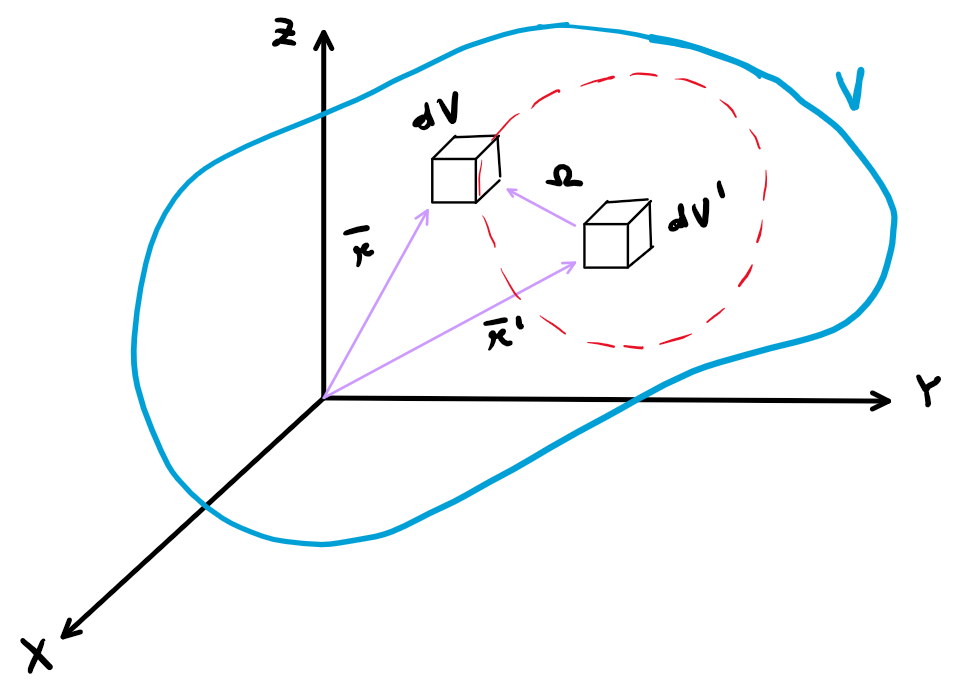
\includegraphics[scale=0.70]{./Figures/P5/integralTransport.png} 
  \caption{Geometry for deriving the integral transport equation.} 
  \label{fig:CP}
\end{figure}

To reach $\mathbf{r}$ from $\mathbf{r}'$, it will take some time. To arrive at $\mathbf{r}$ at time $t$, neutrons would have to leave $\mathbf{r}'$ at a time:
\begin{equation*}
    t' = t - \frac{|\mathbf{r}-\mathbf{r}'|}{v}\;\mathrm{,}
\end{equation*}
where $v$ is the neutron speed.

The number of neutrons coming from $\mathrm{d}V'$ about $\mathbf{r}'$ is from scattering, fission and other sources. The total number of neutrons produced at this point at the appropriate time is:
\begin{equation*}
    q(\mathbf{r}')\mathrm{d}V'\mathrm{d}t'\;\mathrm{,}
\end{equation*}
where $q(\mathbf{r}')$ is the local source rate density. We assume production is isotropic -- otherwise the equations become nightmarish.

The probability that a neutron will fly the appropriate distance $|\mathbf{r}-\mathbf{r}'|$ without colliding along the way is:
\begin{equation*}
    e^{-\Sigma_\mathrm{t}|\mathbf{r}-\mathbf{r}'|}\;\mathrm{,}
\end{equation*}
where $\Sigma_\mathrm{t}$ is the total cross section and we have assumed the medium is homogeneous. If the medium is not homogeneous, we would have to work in terms of the medium's optical depth, giving:
\begin{equation*}
    e^{-\int^{|\mathbf{r}-\mathbf{r}'|}_0\mathrm{d}R\;\Sigma_\mathrm{t}(\mathbf{r'}+\mathbf{\Omega}R)}\;\mathrm{,}
\end{equation*}
where $\mathbf{\Omega}$ is the neutron's flight direction and $R$ is the distance along that direction. We also often rewrite the exponentiated term simply as $\tau(\mathbf{r},\mathbf{r}')$, referred to as the optical distance between the two points.

For neutrons that have been produced by the source, after some time $t - t'$ or after they have travelled a distance $|\mathbf{r}-\mathbf{r}'|$, they will form a spherical shell around the source. This shell will have a volume:
\begin{equation*}
    4\pi|\mathbf{r}-\mathbf{r}'|^2 v\mathrm{d}t'\;\mathrm{.}
\end{equation*}

Putting these expressions all together, the neutron density about $\mathrm{d}V$ due to neutrons about $\mathrm{d}V'$ will be:
\begin{equation*}
    n(\mathbf{r},\mathbf{r}') = \frac{q(\mathbf{r}')e^{-\Sigma_\mathrm{t}|\mathbf{r}-\mathbf{r}'|}\mathrm{d}V'\mathrm{d}t'}{4\pi|\mathbf{r}-\mathbf{r}'|^2v\mathrm{d}t'}\;\mathrm{.}
\end{equation*}
To obtain the actual density of neutrons at the point $\mathbf{r}$, we need to integrate this equation over all of space, giving:
\begin{equation*}
    n(\mathbf{r}) = \int_V q(\mathbf{r}') \frac{e^{-\Sigma_\mathrm{t}|\mathbf{r}-\mathbf{r}'|}}{4\pi|\mathbf{r}-\mathbf{r}'|^2v}\mathrm{d}V'\;\mathrm{,}
\end{equation*}
or, more conventionally, the flux is:
\begin{equation}\label{eq:integral}
    \phi(\mathbf{r}) = \int_V q(\mathbf{r}') \frac{e^{-\Sigma_\mathrm{t}|\mathbf{r}-\mathbf{r}'|}}{4\pi|\mathbf{r}-\mathbf{r}'|^2}\mathrm{d}V'\;\mathrm{.}
\end{equation}

\subsection{Discretisation}

To be able to solve this problem numerically, we need to discretise it. We do so by asserting that space is split up into several homogeneous regions, where region $i$ has volume $V_i$. In each region, we will also have a uniform flux and source (and cross sections), defined as:
\begin{equation*}
    \phi_i = \frac{1}{V_i}\int_{V_i}\mathrm{d}V \phi(\mathbf{r})\;\mathrm{,}
\end{equation*}
\begin{equation*}
    q_i = \frac{1}{V_i}\int_{V_i}\mathrm{d}V q(\mathbf{r})\;\mathrm{.}
\end{equation*}
If we integrate Eq.~\eqref{eq:integral} over volume $V_i$ and multiply by $\Sigma_{\mathrm{t},i}$ we obtain:
\begin{equation}
\begin{split}
    \Sigma_{\mathrm{t},i}\int_{V_i}\mathrm{d}V\phi(\mathrm{r}) = \Sigma_{\mathrm{t},i}\phi_i V_i = \Sigma_{\mathrm{t},i} \int_{V_i}\mathrm{d}V\int_{V}\mathrm{d}V' \frac{q(\mathbf{r'}) e^{-\tau(\mathbf{r},\mathbf{r}')}}{4\pi|\mathbf{r}-\mathbf{r}'|^2} \\
    = \Sigma_{\mathrm{t},i}\sum_j q_j \int_{V_i}\mathrm{d}V\int_{V_j}\mathrm{d}V' \frac{e^{-\tau(\mathbf{r},\mathbf{r}')}}{4\pi|\mathbf{r}-\mathbf{r}'|^2} = \sum_j q_j V_j P_{ij}\;\mathrm{,}
\end{split}
\end{equation}
where we have introduced $P_{ij}$, the collision probability, or the probability that a particle produced in region $i$ will collide in region $j$, defined as:
\begin{equation}
    P_{ij} = \frac{\Sigma_{\mathrm{t},i}}{V_j}\int_{V_i}\mathrm{d}V\int_{V_j}\mathrm{d}V'\frac{e^{-\tau(\mathbf{r},\mathbf{r}')}}{4\pi|\mathbf{r}-\mathbf{r}'|^2}\;\mathrm{.}
\end{equation}
Hence we can write the transport problem as, simply:
\begin{equation}
    \Sigma_{\mathrm{t},i}\phi_i V_i = \sum_j q_j V_j P_{ij}\;\mathrm{,}
\end{equation}
which states that the collision rate in a region is due to the contributions of neutrons born in all regions in the problem. This can be written simply as a matrix multiplication, where $P_{ij}$ is a matrix, acting on the vector $(qV)_j$.

The problem, of course, comes with how to calculate $P_{ij}$. In self-shielding calculations, this is done very approximately as we shall see.

\subsection{Digression on the common use of the collision probability method}

We will be using collision probabilities as a formalism without much meaningful numerics, but the more complete method is important in reactor physics. In particular, after we have done all of our self-shielding calculations, we want to account for spatial effects -- usually this is done on a pin cell level with many groups, followed by calculations on an assembly level with fewer groups.

Where the collision probabilities method (CPM) is most common in reactor physics is in that second step: spatial calculations for single pin cells, for each pin cell type in the reactor. These calculations are often performed with a major approximation: the pins are `circularised' or a Wigner-Seitz cell is constructed, preserving fuel and moderator volumes. This also results in the need to use `white' boundary conditions, rather than the more common reflective or periodic. The reason for this is that calculating collision probabilities in a circular geometry is much more straightforward as the geometry is essentially 1D.

CPM tends not to be applied to larger problems, despite its geometric flexibility. This is due to it producing dense matrices that must be inverted to obtain the flux. Matrix inversion operations are $\mathcal{O}(n^3)$ in time complexity, making the method become intractable as the geometry becomes larger. However, the ray tracing procedures devised for CPM were put to good usage afterwards; they are used by the method of characteristics, which can perform a transport sweep, rather than a direct matrix inversion, and this is now the method of choice for assembly-level lattice physics.
